\begin{refsection}

\chapter{Supplements to Chapter 4}\label{appendix:a4}




M06-L energetically places a quartet state of the cyclic isomer around 1.00 eV lower than a quartet state, the lowest-lying one, of the linear isomers. The lower-lying doublet state is around 0.34 eV less stable than the lowest-lying quartet state.




\begin{figure}[htb!]
	\centering
	\includegraphics[width=0.8\textwidth]{TiGe2-surface-mo6l}
	\caption{Relative energies of the cyclic and linear isomers with many different spin multiplicities at the M06-L functional level of theory.}
	\label{a4fig:RE-linear-cyclic}
\end{figure}






\begin{figure}[htb!]
	\centering
	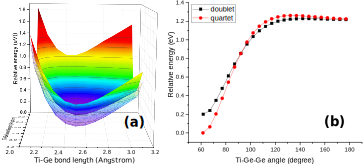
\includegraphics[width=\textwidth]{full-surface}
	\caption{Potential surfaces of the doublet and quartet spin states (a) at the M06-L level of theory with regard to the \ch{Ti-Ge} bond length from 2.1 to 3.1 \AA. The potential surface of the quartet spin state is the lower one (transparent) and the remaining one is the potential surface of the doublet spin state. The energy-profile plot of these two spin states (b) when their geometrical structures change from the cyclic form to the linear one is on the right-hand side. All calculations are done in conjunction with the basis set cc-pVTZ.}
	\label{a4fig:full-surface}
\end{figure}




Figure \ref{a4fig:full-surface}b presents energy profiles of the anionic doublet and quartet when their geometrical structures change from cyclic to linear isomers at the M06-L level of theory. Clearly, the linear isomers of both spin states are more unstable than the cyclic ones with a barrier energy of about 1.20 eV. This barrier energy implies that the linear isomers are believed to not be experimentally populated.











\cleardoublepage

\includebibliography
\printbibliography[heading=subbibliography] % print section bibliography

\end{refsection}